\documentclass{report}
\usepackage[utf8]{inputenc}
\usepackage[T1]{fontenc}
\usepackage{graphicx}
\usepackage[francais]{babel} 
\usepackage{array} 

\title{Etat de l'art}
\author{Projet DUT INFO}
\date{17 Septembre 2013}
\begin{document}
\maketitle
\tableofcontents

\part{Introduction}

\chapter{Principe d'affichage d'une image sur ordinateur}
\section{La carte graphique}
\subsection{Définition}
Une carte graphique, ou carte vidéo, est un périphérique permettant à un ordinateur de communiquer 
avec un écran.\\
\subsection{Composants}
\textbf{GPU} (Graphical Processing Unit) : Processeur graphique, constituant le cœur de la carte graphique, et qui possède des instructions évoluées de traitement d’image. Un GPU est une unité de calcul massivement parallèle.\\\\
\textbf{Mémoire vidéo} (Frame Buffer) : Conserve les images traitées par le GPU avant l’affichage.
\subsection{Fonctionnement en mode texte}
Les premières cartes graphiques datent du début des années 1980, à une époque à laquelle les ordinateurs n'affichaient que du texte à l'écran.\\
Ces cartes ne permettaient d'afficher à l'écran qu'une grille de caractères 
(25 lignes de 80 caractères) prédéfinis qui mesuraient 9x14 pixels chacun. Il était ainsi impossible de modifier directement la valeur d'un pixel.\\
Ce mode de fonctionnement ainsi que la table des caractères utilisables est 
définie par la norme MDA, "Monochrome Display Adapter"\footnote{http://www.seasip.info/VintagePC/mda.html}
du nom de la carte graphique d'IBM qui inaugura cette technologie.\\
Il est à noter que c'est le CPU\footnote{Central Processing Unit : Unité de calcul centrale / Processeur de la machine} qui donnait ses instructions à la carte graphique, celle-ci ne faisant que transmettre les caractères à l'écran.\\
Cette norme est encore utilisée de nos jours, elle permet notamment au BIOS d'afficher des informations au démarrage d'un ordinateur.

\subsection{Fonctionnement en mode graphique}

En 1981 apparait la première carte graphique permettant d'adresser chaque pixel de l'écran indépendamment.
Fabriquée par IBM, cette carte dite CGA, "Color Graphic Adapter" permettait d'utiliser une résolution de 320 par 200 pixels en mode 4 couleurs ou une résolution de 640 par 200 pixels en mode monochrome.\\
Cette carte est une avancée majeure puisqu'elle permet désormais d'afficher n'importe qu'elle forme à l'écran, et plus uniquement des caractères. C'est le début de l'informatique graphique.

\subsection{L'accélération matérielle 2D}

A l'époque, le rôle de la carte graphique se limitait à servir d'intermédiaire entre le CPU et l'écran, c'était le rôle du CPU de définir l'ensemble des pixels à afficher. Par exemple si une application souhaitait tracer une ligne entre deux points A et B, le CPU devait alors calculer la position de chaque pixel composant la ligne avant de demander à la carte graphique d'afficher ceux-ci.\\
Aussi durant les années 1980, avec l'arrivée des interfaces graphiques, les cartes graphiques devinrent de plus en plus performantes dans le but de délester le CPU : elles étaient désormais capables de tracer elles-mêmes des primitives géométriques simples telles que des lignes, des triangles, des rectangles, des cercles, voire de colorier celles-ci d'après les consignes données par le CPU.\\

\subsection{Historique des GPU}
\begin{center}
\begin{tabular}{|c|c|m{0.2\linewidth}|m{0.3\linewidth} |c|}
\hline
Année & Génération & Carte & Application & Bus \\
\hline
1996 & 1 & 3dfx Voodoo & texture mapping et z-buffer & bus PCI\\
\hline
1998 & 2 & GeForce/ Radeon 7500 & Transform\&lighting, multi-texting & bus AGP \\
\cline{1-4}
2001 & 3 & GeForce3/ Radeon 8500 & Programmation sur les sommets (vertex shader)	& \\
\cline{1-4}
2002 & 4 & Radeon 9700/GeForce FX & Programmation sur les pixels (fragment shader)	& \\
\hline
2008 & 5 & GeForce9/ Radeon HD & Compatibilité OpenGL et DirectX,  geometry shader & bus PCIe \\
\hline
\end{tabular}
\end{center}

Les bus PCI(Peripheral Component Interconnect), AGP(Advanced Graphics Port) et  PCIexpress sont des bus local.
Bus local : système de communication entre des cartes d’extension et la carte mère.
Le bus PCIe est une version plus petite et plus performante que le PCI et AGP.


\part{Outils utilisés}

\chapter{OpenGL}

\section{Introduction}
Comme vu précédemment l'affichage d'un contenu à l'écran par ordinateur consiste en un processus de communication entre le processeur , la carte graphique et l'écran. Ces messages, très bas niveau, sont difficilement utilisables directement par les développeurs.

OpenGL est une Interface de Programmation (API) qui définit un moyen de communication entre l'application et la carte graphique.
Cependant il n'existe aucune implémentation "officielle" d'OpenGL, c'est le rôle de chaque constructeur de l'implémenter sur son matériel.  
Elle contient un ensemble de 150 fonctions qui permettent de définir les objets et opérations nécessaires pour rendre un contexte tri-dimensionnel.
L’avantage d'OpenGL est qu’elle est totalement portable avec tous les systèmes d'exploitation. Ceci est dû au fait qu'elle sert plutôt d'intermédiaire entre l'application et le système d'exploitation. OpenGL sert à dessiner le rendu et le communiquer à la carte graphique mais ne gère ni le fenêtrage, ni les évènements. 
La majorité des bibliothèques graphiques utilisées pour créer des fenêtres graphiques gèrent OpenGL, il est donc possible d'utiliser OpenGL dans un contexte SDL, SFML, QT, API Windows.

%Device context ? Rendering context ?

OpenGL est basée sur un principe de primitives : chaque objet est composé de primitives (sommets, faces, polygones) Pour créer un objet, il suffit donc de définir toutes ses primitives.

\newcolumntype{M}[1]{>{\raggedright}m{#1}}

\begin{center}
   \begin{tabular}{| c | M{8cm} |}
   	 \hline
     \verb|GL_POINTS| 			& Dessine un point à chaque n vertex  \tabularnewline
     \hline
     \verb|GL_LINE| 			& Dessine une ligne d’un point n à n+1 \tabularnewline
     \hline
     \verb|GL_LINE_STRIP| 		& Dessine un ensemble de lignes connectées d’un vertex à un autre \tabularnewline
     \hline
     \verb|GL_LINE_LOOP| 		& Même chose que \verb|GL_LINE_STRIP|, mais du dernier vertex, on revient au premier. \tabularnewline
     \hline
     \verb|GL_TRIANGLES| 		& Dessine des triangles avec 3 vertex \tabularnewline
     \hline
     \verb|GL_TRIANGLE_STRIP| 	& Dessine une série de triangles avec les n vertexs définis   \tabularnewline
     \verb|GL_TRIANGLE_FAN| 	& Même chose que \verb|GL_TRIANGLE_STRIP|, sauf que le sommet de chaque triangle est le premier vertex défini \tabularnewline
     \hline
     \verb|GL_QUADS| 			& Dessine un quadrilatère avec 4 vertex \tabularnewline
     \hline
     \verb|GL_QUAD_STRIP| 		& Dessine une série de quadrilatères avec les n vertex définis \tabularnewline
     \hline
     \verb|GL_POLYGON| 			& Dessine un polygône générique dont le nombre de segments \verb|n’est| pas prédéterminé \tabularnewline
     \hline
   \end{tabular}
 \end{center}
 
 \begin{center}
	 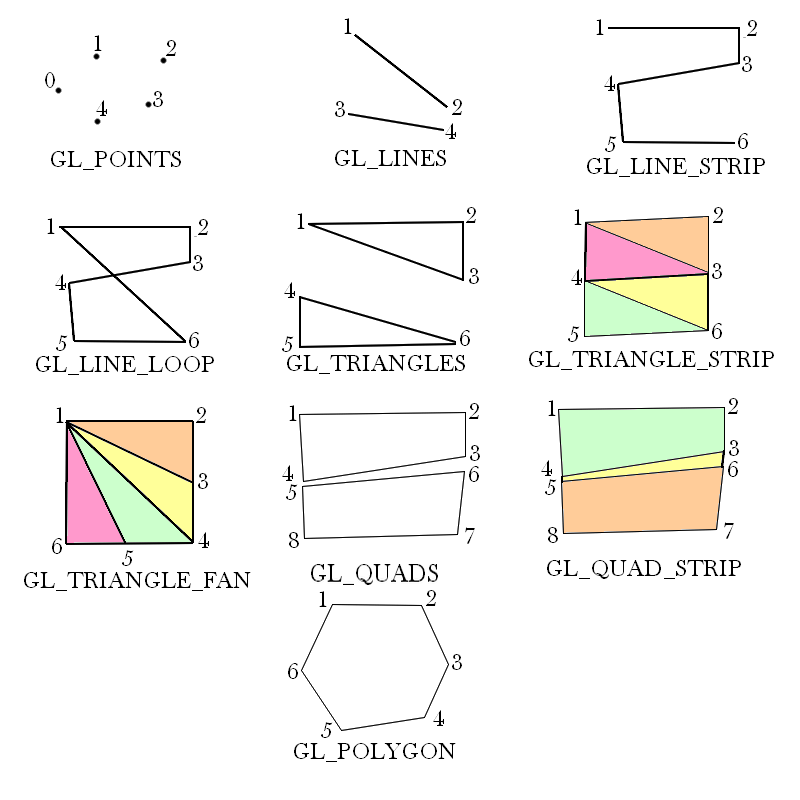
\includegraphics[height=11cm]{img/Primitives}
 \end{center}
\newpage
%Include section Intro


\section{Fonctionnement statique}
\begin{center}
	 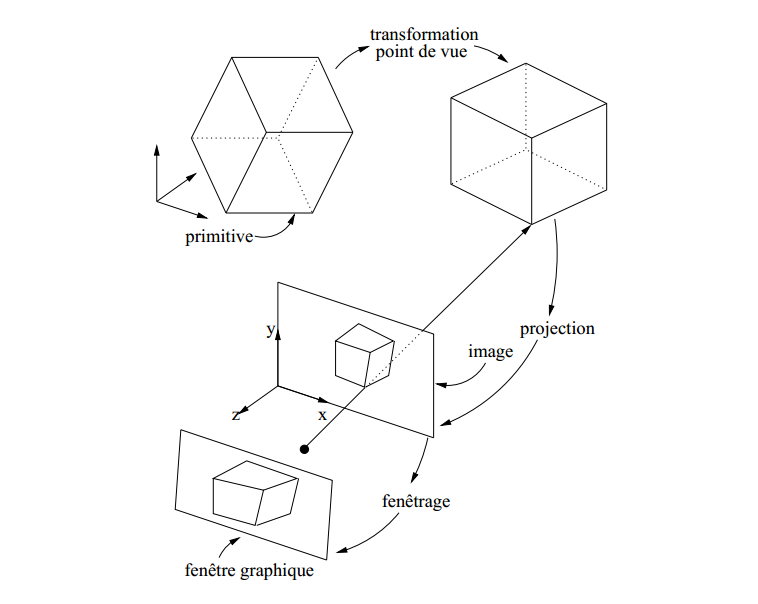
\includegraphics[height=11cm]{img/Fonctionnement}
 \end{center}

La première étape est de définir les primitives des objets à dessiner (x,y,z pour chaque Vertex).
OpenGL dessine une image tampon qui sera soit conservée dans la mémoire vidéo de la fenêtre graphique avant d’être affichée, soit une image tampon intermédiaire, on parle alors de double buffering.

La transformation du point de vue sert à la position du plan image. Elle prend en compte la position de la caméra pour se placer correctement autour de l'objet. Ces modifications sont faites à l'aide de matrices. 

Les primitives sont ensuite projetées sur ce plan en fonction des paramètres que l’on a affecté à la projection. Cette projection peut être spécifiée de deux manières. (Voir Projection)

Au final l’image que l’on obtient est redimensionnée en fonction de la taille de la fenêtre graphique . On parle maintenant de pixels et plus de vertex.
\newpage

\subsection{Primitives}
Tout d'abord, il s'agit de définir chaque objet à modéliser, grâce aux primitives précédemment décrites.

Dans le code, chaque primitives est décrite de la manière suivante:


%//////////////////////////////////
%NE PAS TOUCHER A CE TRUC IMMONDE :)
\begin{tabbing}
XXXX\=XXXX\= \kill

\> \verb|glBegin("type_de_primitive");| \\
\> \> glVertex(x,y,x);\\
\> \> . \\
\> \> . On définit chaque vertex en fonction du type de primitive\\
\> \> . \\
\> \> glVertex(x,y,x);\\
\> glEnd();
\end{tabbing}
%NE PAS TOUCHER A CE TRUC IMMONDE :)
%//////////////////////////////////

\subsection{Transformation de point de vue}
La transformation de point de vue consiste en la modification d'une matrice appelée MODELVIEW. Il faut d'abord signaler à OpenGL que l'on veut modifier cette matrice avec la fonction suivante :

\begin{tabbing}
XXXX\= \kill
\> \verb|glMatrixMode( GL_MODELVIEW );|
\end{tabbing}

Ensuite, on charge la matrice identité, ce qui permet de réinitialiser la matrice en cours, puis définit la caméra.

\begin{tabbing}
XXXX\= \kill
\> \verb|glLoadIdentity( );| \\
\> \verb|gluLookAt(eyeX,eyeY,eyeZ,centerX,centerY,centerZ,upX,upY,upZ);|
\end{tabbing}

La définition de la caméra nécessite 9 paramètres: les 3 premiers pour placer la caméra dans l'espace (x,y,z), les 3 suivants pour définir le point regardé par la caméra (x,y,z) et les trois derniers pour définir quel est l'axe vertical, en général y (On place seulement l'axe voulu à 1 et les autres à 0).\\\\

Il est possible d'effectuer d'autres opérations sur cette matrice, comme une rotation autour d'un des 3 axes ou une translation de vecteurs grâce aux deux fonctions suivantes :

\begin{tabbing}
XXXX\= \kill
\> \verb|glRotatef(angle,x,y,z);| \\\\
Avec l'angle souhaité et x, y et z à 0 ou 1 suivant autour de quel axe on souhaite\\ effectuer la rotation.\\\\
\> \verb|glTranslatef(vX,vY,vZ);|\\\\
Avec vX, vY et vZ les composantes de la translation. 
\end{tabbing}

\subsection{Projection}

La visualisation d'une scène est réalisée par deux types de transformation :

\begin{itemize}
	\item la première qui se situe dans l'espace 3D et qui permet de positionner le point de vue et si nécessaire les éclairages, pour un rendu plus réaliste (la matrice de modélisation $GL\_MODELVIEW$) que nous avons vu précédemment.

	\item la seconde qui consiste à projeter la scène 3D précédemment construite sur un plan en 2D. Sous OpenGL on retrouve deux formes de projection, la projection perspective et la projection orthographique.
\end{itemize}

La projection appliquée suite aux coordonnées des primitives est définie dans OpenGL grâce à une matrice 4x4. L'usage de ces coordonnées permet de représenter les deux types de projections sous la forme de matrices. 

\subsubsection{Perspective}
\begin{center}
	 \includegraphics[height=5cm]{img/Perspective}
 \end{center}
Notre œil perçoit ce qui loin plus petit qu’il ne l’est en réalité. Cette méthode de projection est souvent utilisée en animation, simulation et autre applications où il faudrait un degré de réalisme, comme peut le percevoir notre œil. Pour la définir il faut connaître son centre de projection (frustum), la distance entre ce point et l'objet, et enfin sa direction, qui suivra obligatoirement l’axe z. Sous OpenGL la fonction est : 
\begin{tabbing}
XXXX\= \kill
\> \verb|glFrustum(gauche, droite, bas, haut, proche, éloigné);| \\où les paramètres sont des doubles.
\end{tabbing}


\subsubsection{Orthographique}
\begin{center}
	 \includegraphics[height=7cm]{img/Ortho}
 \end{center}
Dans ce cas précis, l’image doit refléter les mesures de l’objet plutôt que son aspect réel. Contrairement à la projection en perspective la taille du viewing volume ne change pas, la distance depuis la caméra n’affecte pas la mesure de l’objet. Sous OpenGL la fonction est : 
\begin{tabbing}
XXXX\= \kill
\> \verb|glOrtho(gauche, droite, bas, haut, proche, éloigné);| \\où les paramètres sont des doubles.
\end{tabbing}

\subsection{Image Finale}

%A compléter

\newpage%Include section Fonctionnement Statique

\section{Fonctionnement dynamique}
%SHADERS

\subsection{Principe du Shader}

Le fonctionnement dynamique du pipeline graphique se différencie du fonctionnement statique par l'utilisation de shaders.
Comme expliqué précédemment les shaders sont de petits programmes écrits dans un langage spécifique : avec OpenGL, le langage utilisé est le GLSL.\\
Ils sont compilés à l'éxécution du programme OpenGL, et executés pour chaque vertex (Vertex Shader) et chaque pixel (Pixel Shader).
Ils remplacent les calculs de matrices gérés par défaut dans le fonctionnement statique d'OpenGL. C'est-à-dire qu'il faut implémenter ces calculs dans les shaders. L'intérêt est qu'il est possible d'adapter ces calculs pour satisfaire certains besoins de l'application. D'autant plus que les shaders sont exécutés par la carte graphique(GPU), qui est capable de répartir les opérations sur toutes les unités de calculs.

\subsection{Utilisation des shaders}

Il est plus ou moins aisé d'implémenter les shaders dans un programme OpenGL, suivant la bibliothèque graphique utilisée.
Nous prenons l'exemple de la SFML:\\

\begin{tabbing}
XXXX\=XXXX\= \kill\\
\> //On déclare un objet de type Shader\\
\> \verb|sf::Shader shader;|\\
\\
\>//Puis on charge les fichiers shaders\\
\> \verb|if (!shader.loadFromFile("vertex_shader.vert", "fragment_shader.frag"))|\\
\> \verb|{|\\
\> \>\verb|//error...|\\
\> \verb|}|\\
\end{tabbing}

Pour utiliser le shader il faut l'activer avant de dessiner et le désactiver quand on en a plus besoin.


\begin{tabbing}
XXXX\=XXXX\= \kill\\
\> // On active le shader\\
\> \verb|sf::Shader::bind(&shader);|\\
\\
\> ....\\
\> //On dessine nos entités OpenGL ....\\
\> ....\\
\\
\> // On désactive le shader\\
\> \verb|sf::Shader::bind(NULL);|\\
\end{tabbing}

\subsection{Exemple de Shader}
\subsubsection{Vertex Shader}

\begin{tabbing}
XXXX\=XXXX\= \kill\\
\> \verb|uniform float a;|\\
\> \\
\> \verb|void main(){|\\
\> \\
\>\> \verb|vec4 vertex = gl_Vertex;| \\
\> \\
\>\> \verb|vertex.y = vertex.y + a*cos(vertex.y)| \\
\> \\
\>\> \verb|gl_Position = gl_ModelViewProjectionMatrix * vertex;|\\
\> \\
\>\> \verb|// transforme les coordonnées de texture|\\
\>\> \verb|gl_TexCoord[0] = gl_TextureMatrix[0] * gl_MultiTexCoord0;|\\
\> \\
\>\> \verb|// transmet la couleur|\\
\>\> \verb|gl_FrontColor = gl_Color;|\\
\> \verb|}|\\
\end{tabbing}


\subsubsection{Pixel Shader}

\begin{tabbing}
XXXX\=XXXX\= \kill\\
\> \verb|uniform float a;| \\
\> \\
\> \verb|void main(){|\\
\> \\
\> \verb|gl_Position = gl_ModelViewProjectionMatrix * gl_Vertex;|\\
\> \\
\> \verb|}|\\
\end{tabbing}%Include section Fonctionnement Dynamique



\chapter{Bibliothèque de rendu 3D}
 \section{Introduction}
incomplet...

%A compléter
\part{Problèmes Rencontrés}

\chapter{Optimisation}
\newpage
\end{document}